%%%%%%%%%%%%%%%%%%%%%%%%%%%%%%%%%%%%%%%%%
% University/School Laboratory Report
% LaTeX Template
% Version 3.1 (25/3/14)
%
% This template has been downloaded from:
% http://www.LaTeXTemplates.com
%
% Original author:
% Linux and Unix Users Group at Virginia Tech Wiki 
% (https://vtluug.org/wiki/Example_LaTeX_chem_lab_report)
%
% License:
% CC BY-NC-SA 3.0 (http://creativecommons.org/licenses/by-nc-sa/3.0/)
%
%%%%%%%%%%%%%%%%%%%%%%%%%%%%%%%%%%%%%%%%%

%----------------------------------------------------------------------------------------
%	PACKAGES AND DOCUMENT CONFIGURATIONS
%----------------------------------------------------------------------------------------

\documentclass{article}

\usepackage[version=3]{mhchem} % Package for chemical equation typesetting
%\usepackage{siunitx} % Provides the \SI{}{} and \si{} command for typesetting SI units
\usepackage{graphicx} % Required for the inclusion of images
\usepackage{natbib} % Required to change bibliography style to APA
\usepackage{amsmath} % Required for some math elements 
\usepackage{hyperref}
\usepackage[a4paper,margin=0.5in]{geometry}
\setlength\parindent{0pt} % Removes all indentation from paragraphs

\renewcommand{\labelenumi}{\alph{enumi}.} % Make numbering in the enumerate environment by letter rather than number (e.g. section 6)

%\usepackage{times} % Uncomment to use the Times New Roman font

%----------------------------------------------------------------------------------------
%	DOCUMENT INFORMATION
%----------------------------------------------------------------------------------------

\title{Gate Detection} % Title

\author{Philipp \textsc{Duernay}} % Author name

\date{\today} % Date for the report

\begin{document}
\maketitle
% If you wish to include an abstract, uncomment the lines below
% \begin{abstract}
% Abstract text
% \end{abstract}

%----------------------------------------------------------------------------------------
%	SECTION 1
%----------------------------------------------------------------------------------------

\section{Recap}
In the last meeting from 07.03.2018 several next steps were defined:
\begin{enumerate}
	\item \textbf{Finish labeling of video to quantify results better}
	\item \textbf{Measure speed with tensorflow profiling}
	\item \textbf{Try to make ssd work on gate data}
	\item \textbf{Investigate sequence based approach}
	\item \textbf{Read on transfer learning between synthetic and real data}
	\item \textbf{Generate training data similar to MAVLab set}
\end{enumerate}

\section{Data}

So far good results could only be achieved when testing on the synthetic data. On the real data some detections could be made on the video of last years race (\textit{ethset}) but the results were really poor on the images taken in the basement of the MAVLab(\textit{mavset}). In \autoref{comparison} the different datasets are compared.
\begin{table}[]
	\centering
	\caption{Dataset Comparison}
	\label{comparison}
	\begin{tabular}{p{3cm}|p{4cm}|p{4cm}|p{4cm}}
					&  training set (\textbf{so far})& \textit{ethset} 					& \textit{mavset}	\\
					\hline
		Resolution 	&  416x416								  &  1280x720 								&  180x315			\\
		\hline
		Lense		&  Pinhole (might vary dep. on background)&  Rectified							&  Fisheye		  	\\
		\hline
		Lighting	&  dep. background, sun light on gates	  &  multiple directed strong sources	&  multiple directed weak sources\\ 
		\hline
		Scene		&  Indoor/Outdoor/ City/Nature			  &  Indoor industrial bright			&  Indoor basement dark	\\
		\hline
		Gates		&  subset of 3d models of IROS2016/17	  &  IROS 2017							&  built by MAVLab (black pole)	\\
		\hline
		Gate Placement & multiple gates out of context 		  &  multiple according to race court	&  single gate		\\
		\hline
		Blur		&  Gaussian Blur (Image aug)			  &  Motion blur						&  Motion blur 	\\
		\hline
		Noise		&  Gray noise (Image aug)				  &  Camera noise +artifacts			&  Camera noise + artifacts	\\
		\hline
	\end{tabular}
\end{table}

The following lists methods investigated to cope between the shift from training to test images. When and how they are applied is listed in section Evaluation.

\begin{itemize}
	\item \textbf{Resolution}. We change the resolution of the network to fit to the test set. As long as the architecture is not changed this also yields a new grid and potentially the aspect ratios of the anchor boxes are not suitable for the data anymore. To get new aspect ratios we follow the approach of YoloV2 where these parameters are found applying a k-means clustering on the bounding boxes of the training set.
	
	\item \textbf{Lense}. To mimic the distortion effects of a fisheye lense a barrel distortion model (Browns distortion model) from the image center is applied to training images. The parameters can be estimated using camera calibration techniques. Unfortunately, the connection to the bebop camera was not possible even with multiple PCs/laptops. Michael sent images he used for calibration however, on those the estimated model did not lead to sufficient accuracy. Hence, the parameters had to be estimated visually.
	
	\item \textbf{Lighting}. We scale the v-channel in hsv-space to change the lighting of an image. Each image in training is scaled randomly (uniform) within a certain range. To cope with different contrasts batch normalization is applied after each convolutional layer (part of the original architecture).
	
	\item \textbf{Gates} As the \text{mavset} also contains gates that have a black pole, another 3d model is added to the training set. That is an orange square without any pole.
	
	\item \textbf{Gate Placement} To get a more realistic setting the backgrounds are chosen more carefully such that the gates are more aligned with the scene. Better placement is also achieved by applying Gaussian blurring only along the gate.
	
	\item \textbf{Blur} Especially the \textit{mavset} contains strong motion blur also from radial movements. The radial blur is hard to model however linear blur can be modeled using a 1d-Gaussian filter along the movement axis on the training images.
	
	\item \textbf{Noise} Next to gray/colour noise added from a Gaussian distribution another method is applied ot mimic some image artifacts. Location in the image are sampled randomly (uniform) and within a certain window size all pixels are replaced by their collective mean.
	

\end{itemize}

%
\section{SSD}

SSD still does work properly. On the Pascal VOC some objects are detected but its very inaccurate. The training converges to a minimum, usually without really increasing the detection performance. However, tensorflow-object-detection is an extension for tensorflow that contains ssd. We can use it to test whether is worth for further debugging.

\section{Evaluation}

\subsection{Experiment I}

In this experiment we tune the model to fit the mavset to see whether this gives better results. The resolution is changed to 180x320 which gives a new grid of (5,10), anchor box ratios are found using kmeans clustering. 

The training set contain 25 000 samples and is similar to the one described in \autoref{comparison} however several additional methods are applied:
\begin{itemize}
	\item Brightness augmentation. The v-value in hsv-space is scaled between 0.5 to 2.0. Where the scale factor is sampled from a uniform distribution for each image when training.
	\item Gray noise is added to the 0.255 pixel range from a Gaussian with $\mu =0, \sigma=10$, during training.
	\item There is a 50\% chance of flipping the image vertically.
	\item There is a 20\% chance of shifting the image vertically between a factor of -0.3 and 0.3.
	\item "Artifacts" are applied to 0.5 \% of the image.
	\item The gates are IROS2016 gates plus an orange square.
\end{itemize}

Method I does not apply a distortion model, Method II applies a barrel distortion with $k_1 = 0.1, p_1=0.1$.  The results can be seen in \autoref{fig:mavset} and \autoref{fig:ethset}, they are labelled "Distorted", "Not Distorted".

We see generally quite poor results on the mavset such that the recall never exceeds 0.25. With caution it looks like distorting the image actually improved performance. However, yolov2 does not seem to predict anything correctly. 

Both models perform relatively well on the ethset. We see how the distortion makes the performance slightly worse which makes sense as the images of the ethset are rectified. We can conclude the reason for the bad performance on the mavset lays in the shift between training and test data.

\subsection{Experiment II}

One big difference between the training data so far and the mavset is the background. In this experiment the backgrounds are taken from empty images of the testset. This can't be done for the real model but we can see whether a more suitable background will improve the performance. 

In total 44 backgrounds are chosen and a training set of 10000 samples is generated. To place the images better in the scene Gaussian blurring with a kernel of (7,7) and $\sigma = 3$ is applied only along the gate. To be robust against light changes brightness scaling within 0.5 and 2.0 is applied to the gate pixels. The results can be seen in \autoref{fig:mavset} and \autoref{fig:ethset}, they are labelled "Cyberzoo Background".

We see a big boost in performance for both models on the mavset. Even yolov2 now gets good results. This is achieved with only 44 different background images. Of course the model is totally overfitted to the mav scene. However, we can conclude that the scene/gate placement is a key factor for performance.

On the ethset on the other hand the performance drops quite a bit. This is very expected as the training data has only the cyberzoo images as a background. For that fact the performance drop is surprisingly low.

\subsection{Experiment III}

In the last experiment the training data was totally tuned to the mavset. In this experiment we want to see whether we can generalize the training data to get better results on both datasets.

To the dataset of the previous experiment a new set of 15000 samples is added. The backgrounds are now chosen more carefully. They come from industrial scene where the point of view is aligned with how a drone/person could see it. The gate placement is similar to experiment II. The image augmentation is similar to Experiment I. The same distortion model is applied. The results can be seen in \autoref{fig:mavset} and \autoref{fig:ethset} as "Cyberzoo + Industrial".

We see a slight breakdown in performance on the mavset which was kind of expected since we tried to generalize the model. Still the performance is much higher than when only using random backgrounds. 

Surprisingly the performance on the ethset drops even further. This is behaviour that should be investigated further. A reason could be the fact that the ethset is not distorted. However, in Experiment I there was not such a big measurable effect when distorting the images. Still we should see how the performance changes when applying the same distortion model on the test data as on the training data.


\begin{figure}[h]
	\centering
	\begin{minipage}{0.45\textwidth}
		\centering
	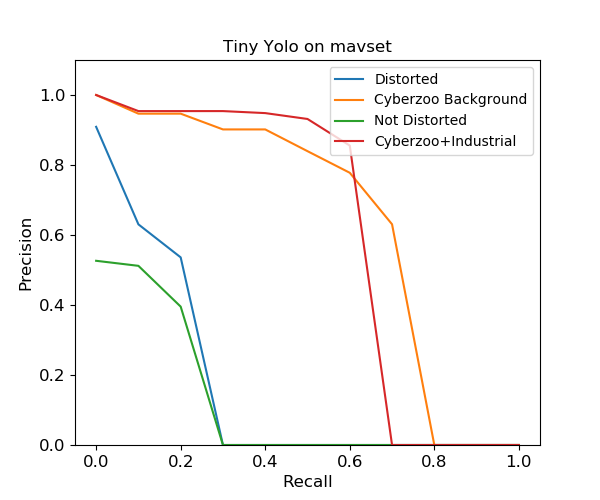
\includegraphics[width=\textwidth]{fig/tiny}
	\end{minipage}
	\begin{minipage}{0.45\textwidth}
		\centering
	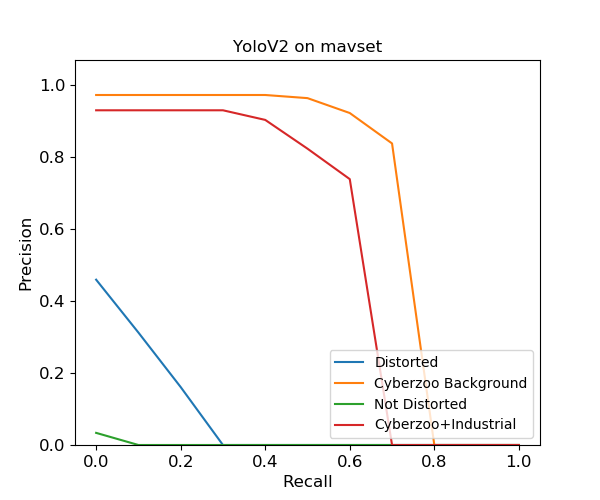
\includegraphics[width=\textwidth]{fig/yolov2}
	\end{minipage}
	\label{fig:mavset}
	\caption{The figure shows precision-recall curves in terms of \textbf{overall} bounding box detections. This is in contrast to the previous reports where the plots showed an average across the images. The method was chosen as especially in the mavset a lot of images are empty, leading to a precision and recall of 0 even if the model correctly did not predict anything.}
\end{figure}

\begin{figure}[h]
	\centering
	\begin{minipage}{0.45\textwidth}
		\centering
		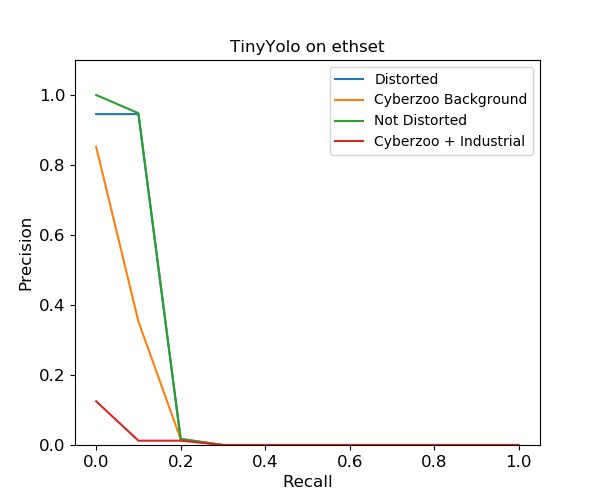
\includegraphics[width=\textwidth]{fig/tiny_eth}
	\end{minipage}
	\begin{minipage}{0.45\textwidth}
		\centering
		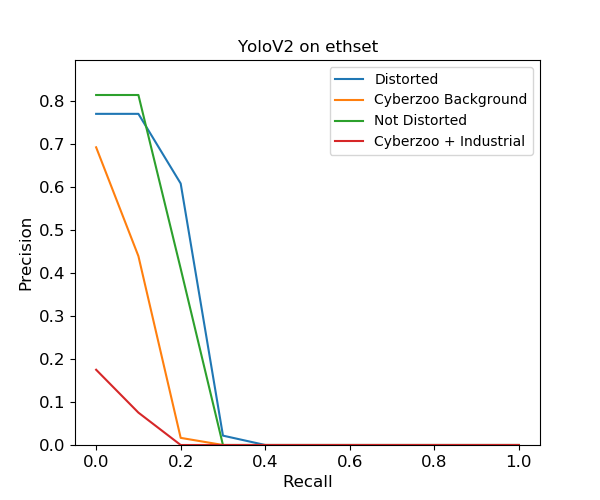
\includegraphics[width=\textwidth]{fig/yolov2_eth}
	\end{minipage}
	\label{fig:ethset}
	\caption{The figure shows precision-recall curves in terms of \textbf{overall} bounding box detections. This is in contrast to the previous reports where the plots showed an average across the images. The method was chosen as especially in the mavset a lot of images are empty, leading to a precision and recall of 0 even if the model correctly did not predict anything.
	The dataset comes from the video of ETH last year. It is a very challenging set containing 150 samples, where especially the first half contains very difficult gates and a lot of gates are far in the background. This performance was achieved by applying the model to the second half of the track so its 77 images.}
\end{figure}


\section{Conclusion}

\begin{itemize}
	\item The backgrounds of the training data have a big effect on performance. If train and test backgrounds are too far apart the model does not work at all.
	\item Creating a general model that performs equally well on both datasets could not be achieved by simply merging two training sets.
\end{itemize}

\section{Next Steps}
\begin{enumerate}
		\item Shift model tuning/sequence based approach/ better localization to the back and investigate pipeline from generated to real images
		\item Generate training data from simulator
		\item Use ssd from tensorflow-objectdetection-toolkit.
		\item Read on transfer learning between synthetic and real data

\end{enumerate}


%----------------------------------------------------------------------------------------


%----------------------------------------------------------------------------------------
%	BIBLIOGRAPHY
%----------------------------------------------------------------------------------------

\bibliographystyle{abbrv}

\bibliography{literature}

%----------------------------------------------------------------------------------------


\end{document}\grid
